As for the use of light microscopes, there are several techniques and configurations which are achieved by varying the amount of lenses and light sources: bright-field, dark-field, phase-contrast, differential interference and fluorescence \cite{roane2009microscopic}. In this work, the \emph{stereomicroscopy}, \emph{bright-field microscopy} and the \emph{z-stacking} techniques are used in order to capture images. As stated by \citeonline{lawlor2019introduction}, images in bright-field microscopy are characterized by the contrast between the sample and the bright white background, generated by transmitted light. It is commonly used in pathology and histology fields for imaging fixed cells and tissues to reveal their structure, shape, and organization. The amount of light should be controlled, since the sample might suffer substantial changes, e.g. the chlorophyll molecules when illuminated by UV and visible light suffer irreversible breakdown (photodegradation) and generate other photoproducts \cite{petrovic2017clorophyll}. The \autoref{fig:bright-field_microscopy} provides an example of bright-field microscopy image.

\begin{figure}[htb]
	\centering
	\caption{\label{fig:bright-field_microscopy} Example of bright-field microscopy of a bone tissue.}
	\begin{center}
	    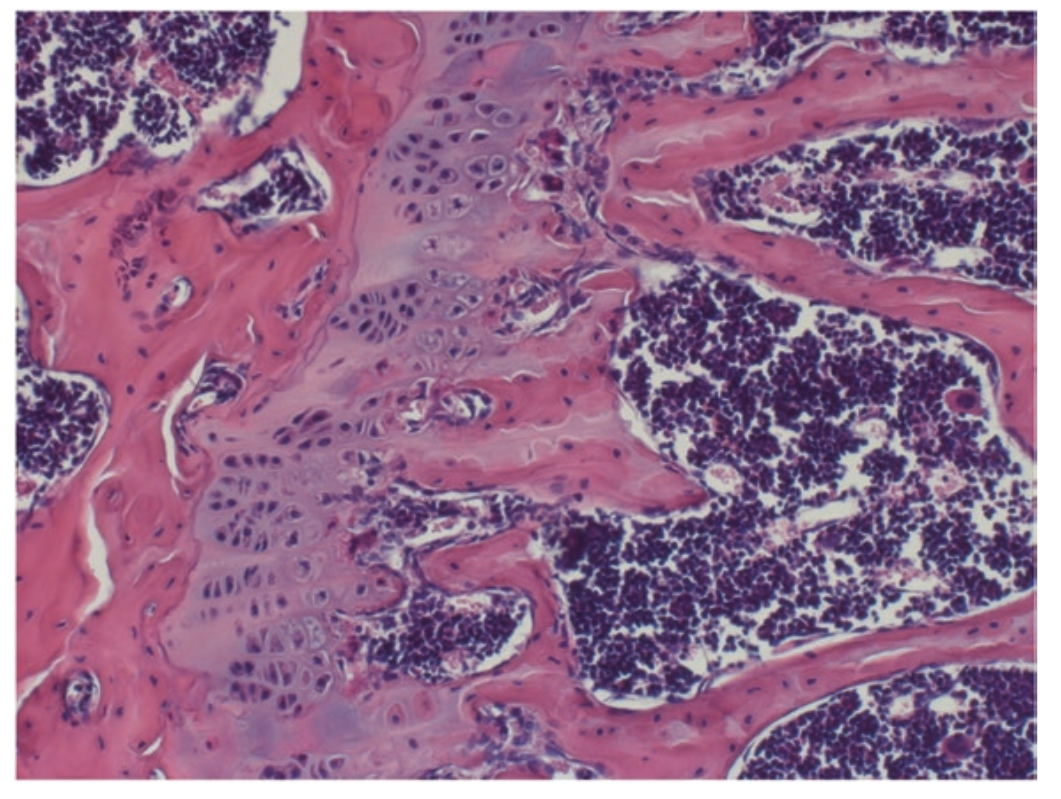
\includegraphics[scale=0.3]{images/bright-field_microscopy.png}
	\end{center}
	\centering
    \fdireta{lawlor2019introduction}
\end{figure}

The z-stacking is a procedure to capture images in different positions concerning the $z$ axis, named slices, which may be applied to many different techniques to create a pseudo 3D image of the sample and consequently retrieve depth information about the specimen \cite{lawlor2019introduction}. The distance between each slice is dictated by the technique, either manually or automatically, and the focus needs to be adjusted at each slice. Next, the images must be aligned before any analysis is conducted. \autoref{fig:z-stack_example} represents a z-stacking example.

\begin{figure}[H]
	\centering
	\caption{\label{fig:z-stack_example} Z-stack images of yeast cells, acquired in positions under the focal plane (-15, -10 and -5 $\mu m$), exactly on it (0 $\mu m$) and above it (5, 10 and 15 $\mu m$).}
	\begin{center}
	    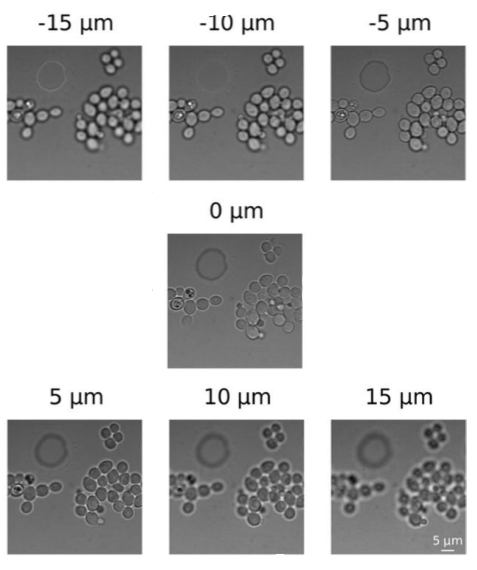
\includegraphics[scale=0.5]{images/z-stack.png}
	\end{center}
	\centering
    \fadaptada{wei2018neural}
\end{figure}